\documentclass{beamer}
\usetheme{Berlin}
%\usecolortheme{dolphin}
\usepackage[utf8]{inputenc}
\usepackage[T1]{fontenc}

\usepackage{csvsimple}
\usepackage{graphicx}
\graphicspath{ {./img/} } % Path relative to the main .tex file 
\newcommand{\fg}[2]{%
  \begin{center}
      \includegraphics[width = #1\textwidth]{#2}%
  \end{center}
}

\usepackage{verbatim}
\usepackage{cancel}
\usepackage{amsmath, amssymb, amsthm}

\title{Regressione Lineare e Anova}

\subtitle{Progetto di Inferenza Statistica}

\author{ D. Bonalumi, M. Bonfadini, L. Colangelo, L. Cossiga}

\institute{Politecnico di Milano}

\date{4 Luglio 2023}

\begin{document}

\frame{\titlepage}

\begin{frame}
    \frametitle{Obiettivo}
    Vogliamo spiegare il livello di felicità di un paese a partire da una serie di indici.
\end{frame}

\begin{frame}
    \frametitle{Table of Contents}
    \tableofcontents
\end{frame}

\section{Presentazione del dataset}

\begin{frame}
    \frametitle{Dataset: The Economics of Happiness (TEH) 2019}
    Fonte: 
    \smallskip
    \footnotesize{\texttt{https://www.kaggle.com/datasets/the-economics-of-happiness-teh}}
\end{frame}

\begin{frame}
    \frametitle{Covariate presenti}
	\begin{itemize}
	\item \texttt{Country}
	\item \texttt{Happiness.rank}
	\item \texttt{Happines.Score}
	\item \texttt{GDP.per.capita}
	\item \texttt{Social.support}
	\item \texttt{Healthy.life}
	\item \texttt{Freedom}
	\item \texttt{Generosity}
	\item \texttt{Corruption}
	\item \texttt{Year}
	\end{itemize}
	con 156 osservazioni.
\end{frame}

\begin{frame}
    Iniziamo rimovuendo le variabili superflue:
    \begin{equation*}
    \xcancel{\texttt{Country}} \qquad \xcancel{\texttt{Happiness.rank}}\qquad\xcancel{\texttt{Year}}
    \end{equation*}
\end{frame}

\begin{frame}[fragile]
    \frametitle{Sono presenti `Not Available'?}
    \tiny
    \begin{verbatim}
                     Country GDP.per.capita Social.support Healthy.life Freedom Generosity Corruption
71                   Moldova          0.685          1.328        0.739   0.245      0.181         NA
82                    Greece          1.181          1.156        0.999   0.067         NA      0.034
112                  Somalia             NA          0.698        0.268   0.559      0.243      0.270
135                Swaziland          0.811          1.149           NA   0.313      0.074      0.135
154              Afghanistan          0.350          0.517        0.361      NA      0.158      0.025
155 Central African Republic          0.026             NA        0.105   0.225      0.235      0.035
    \end{verbatim}

    \normalsize Dato che la distribuzione dei \textit{missing values} è uniforme tra le covariate, possiamo procedere con l'eliminazione delle soprastanti righe.
\end{frame}

\begin{frame}
    \fg{1}{ggpairs1}
\end{frame}

% 2

\section{Modello di regressione lineare}

\begin{frame}[fragile]
	Generiamo il modello lineare con risposta \texttt{Happiness.Score}:

	\tiny
	\begin{verbatim}
Call:
lm(formula = Happiness.Score ~ ., data = Data)

Residuals:
    Min      1Q  Median      3Q     Max 
-1.7416 -0.3528  0.0511  0.3726  1.2817 

Coefficients:
               Estimate Std. Error t value Pr(>|t|)    
(Intercept)      1.6813     0.2341   7.182 3.46e-11 ***
GDP.per.capita   0.8016     0.2314   3.464 0.000702 ***
Social.support   1.2245     0.2541   4.819 3.64e-06 ***
Healthy.life     1.0472     0.3773   2.776 0.006249 ** 
Freedom          1.4086     0.3939   3.576 0.000477 ***
Generosity       0.4812     0.5077   0.948 0.344802    
Corruption       0.9547     0.5585   1.709 0.089561 .  
---
Signif. codes:  0 ‘***’ 0.001 ‘**’ 0.01 ‘*’ 0.05 ‘.’ 0.1 ‘ ’ 1

Residual standard error: 0.5368 on 143 degrees of freedom
Multiple R-squared:  0.7705,    Adjusted R-squared:  0.7609 
F-statistic: 80.01 on 6 and 143 DF,  p-value: < 2.2e-16
	\end{verbatim}
\end{frame}

\begin{frame}
	\frametitle{Controlliamo normalità e omoschedasticità dei residui}
	L'omoschedasticità è rispettata e lo Shapiro test non rifiuta la normalità con un p-value di 0.1296
	\begin{figure}
	   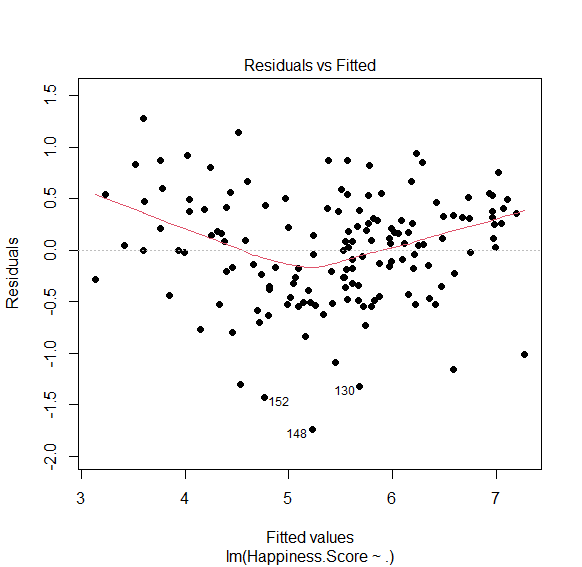
\includegraphics[width=0.4\textwidth]{Awhic1}
	   \hfill
	   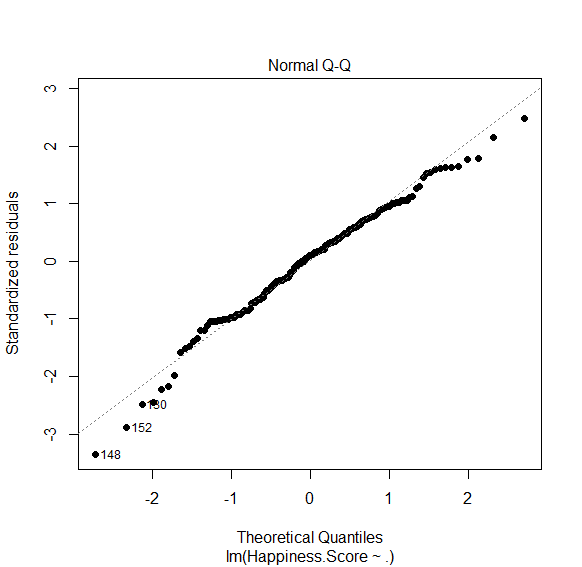
\includegraphics[width=0.4\textwidth]{Bwhic2}
	\end{figure}
\end{frame}

\begin{frame}
    \frametitle{Influential Plot}
    \fg{1}{diagram-20230701}
\end{frame}

\begin{frame}[fragile]
    Eliminiamo i tre punti influenti e ripetiamo il modello:

    \tiny
    \begin{verbatim}
Call:
lm(formula = Happiness.Score ~ ., data = Data)

Residuals:
     Min       1Q   Median       3Q      Max 
-1.76513 -0.33250  0.04344  0.32367  1.15855 

Coefficients:
               Estimate Std. Error t value Pr(>|t|)    
(Intercept)      1.7936     0.2249   7.976 4.69e-13 ***
GDP.per.capita   0.6859     0.2231   3.075  0.00253 ** 
Social.support   1.1086     0.2440   4.544 1.18e-05 ***
Healthy.life     1.1303     0.3609   3.132  0.00211 ** 
Freedom          1.5624     0.3776   4.138 5.99e-05 ***
Generosity       0.3489     0.4880   0.715  0.47578    
Corruption       1.4853     0.5553   2.675  0.00836 ** 
---
Signif. codes:  0 ‘***’ 0.001 ‘**’ 0.01 ‘*’ 0.05 ‘.’ 0.1 ‘ ’ 1

Residual standard error: 0.5115 on 141 degrees of freedom
Multiple R-squared:  0.7829,    Adjusted R-squared:  0.7737 
F-statistic: 84.76 on 6 and 141 DF,  p-value: < 2.2e-16
    \end{verbatim}
\end{frame}

\begin{frame}
    \frametitle{Controlliamo normalità e omoschedasticità dei residui}
    L'omoschedasticità è rispettata e lo Shapiro test non rifiuta la normalità con un p-value di 0.1128
    \begin{figure}
       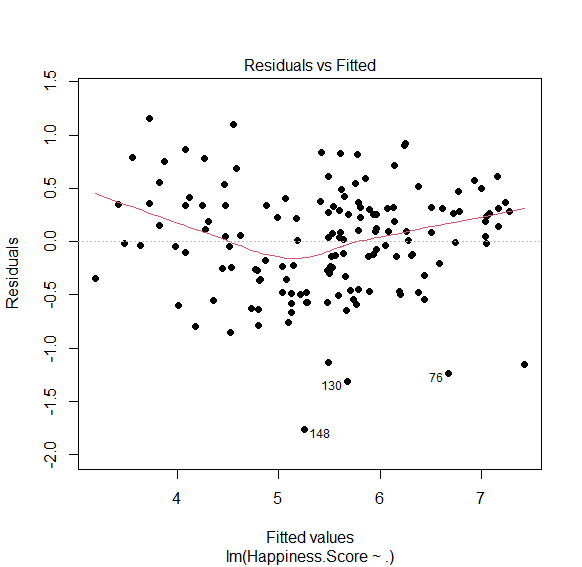
\includegraphics[width=0.4\textwidth]{Awhic2}
       \hfill
       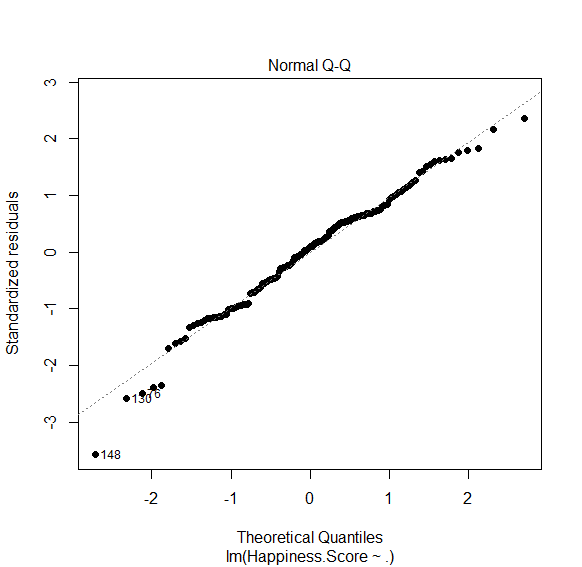
\includegraphics[width=0.4\textwidth]{Bwhic3}
    \end{figure}
\end{frame}

% 3

\section{Selezione delle variabili}  

\begin{frame}[fragile]
    \frametitle{Selezione manuale}
    Per quanto osservato prima, proviamo a costruire un modello senza la variabile \texttt{Generosity}:

    \tiny
    \begin{verbatim}
Coefficients:
               Estimate Std. Error t value Pr(>|t|)    
(Intercept)      1.8484     0.2110   8.759 5.35e-15 ***
GDP.per.capita   0.6654     0.2208   3.013  0.00306 ** 
Social.support   1.1047     0.2435   4.537 1.21e-05 ***
Healthy.life     1.1276     0.3602   3.130  0.00212 ** 
Freedom          1.6184     0.3687   4.389 2.20e-05 ***
Corruption       1.6081     0.5272   3.050  0.00273 ** 
---
Signif. codes:  0 ‘***’ 0.001 ‘**’ 0.01 ‘*’ 0.05 ‘.’ 0.1 ‘ ’ 1

Residual standard error: 0.5107 on 142 degrees of freedom
Multiple R-squared:  0.7822,    Adjusted R-squared:  0.7745 
F-statistic:   102 on 5 and 142 DF,  p-value: < 2.2e-16
    \end{verbatim}

    \normalsize 
    $R^2_{adj}$ passa da $0.7737$ a $0.7745$, il p-value dello Shapiro test è pari a $0.09742$ 
    % quindi non rifiutiamo la normalità con un livello $\alpha=5\%$
\end{frame}

\begin{frame}[fragile]
    Ripetiamo il processo, eliminando \texttt{GDP.per.capita}:

    \tiny
    \begin{verbatim}
Coefficients:
               Estimate Std. Error t value Pr(>|t|)    
(Intercept)      1.6118     0.2013   8.005 3.74e-13 ***
Social.support   1.3655     0.2339   5.838 3.41e-08 ***
Healthy.life     1.8270     0.2831   6.453 1.59e-09 ***
Freedom          1.5896     0.3788   4.196 4.75e-05 ***
Corruption       1.8512     0.5355   3.457 0.000719 ***
---
Signif. codes:  0 ‘***’ 0.001 ‘**’ 0.01 ‘*’ 0.05 ‘.’ 0.1 ‘ ’ 1

Residual standard error: 0.5249 on 143 degrees of freedom
Multiple R-squared:  0.7682,    Adjusted R-squared:  0.7617 
F-statistic: 118.5 on 4 and 143 DF,  p-value: < 2.2e-16
    \end{verbatim}

    \normalsize 
    $R^2_{adj}$ passa da $0.7745$ a $0.7617$, ora il p-value dello Shapiro test sale a $0.6547$
\end{frame}

\begin{frame}[fragile]
    Infine, eliminiamo \texttt{Corruption}:

    \tiny
    \begin{verbatim}
Coefficients:
               Estimate Std. Error t value Pr(>|t|)    
(Intercept)      1.5828     0.2087   7.585 3.76e-12 ***
Social.support   1.2698     0.2410   5.270 4.88e-07 ***
Healthy.life     2.0744     0.2842   7.300 1.79e-11 ***
Freedom          2.0075     0.3725   5.390 2.82e-07 ***
---
Signif. codes:  0 ‘***’ 0.001 ‘**’ 0.01 ‘*’ 0.05 ‘.’ 0.1 ‘ ’ 1

Residual standard error: 0.5445 on 144 degrees of freedom
Multiple R-squared:  0.7489,    Adjusted R-squared:  0.7436 
F-statistic: 143.1 on 3 and 144 DF,  p-value: < 2.2e-16
    \end{verbatim}

    \normalsize 
    $R^2_{adj}$ passa da $0.7617$ a $0.7436$, p-value dello Shapiro test: 0.5452
\end{frame}

\begin{frame}
    \frametitle{RECAP}
    Ripercorriamo il processo di selezione, andando ad osservare anche il relativo indice di Akaike per ogni modello:
\end{frame}

\begin{frame}
    \begin{equation*}
    {\renewcommand*{\arraystretch}{1.4}
    \begin{array}{ccc}
    {\texttt{GDP.per.capita}} & {\texttt{Social.support}} & {\texttt{Healthy.life}} \\
    {\texttt{Freedom}}        & {\texttt{Generosity}}     & {\texttt{Corruption}}
    \end{array}}
    \end{equation*}

    \begin{figure}[h]
    \centering
    {\renewcommand\arraystretch{1.6}
    \begin{tabular}{|c|c|c|}
    \hline
    $R^2_{adj}$ & AIC & Shapiro test p-value \\
    \hline
    0.7737  & 230.4169 & 0.1128 \\
    \hline
    \end{tabular}}
    \end{figure}
\end{frame}

\begin{frame}
    \begin{equation*}
    {\renewcommand*{\arraystretch}{1.4}
    \begin{array}{ccc}
    {\texttt{GDP.per.capita}} & {\texttt{Social.support}} & {\texttt{Healthy.life}} \\
    {\texttt{Freedom}}        & \xcancel{\texttt{Generosity}}     & {\texttt{Corruption}}
    \end{array}}
    \end{equation*}

    \begin{figure}[h]
    \centering
    {\renewcommand\arraystretch{1.6}
    \begin{tabular}{|c|c|c|}
    \hline
    $R^2_{adj}$ & AIC & Shapiro test p-value \\
    \hline
    0.7745  & 228.9526 & 0.09742 \\
    \hline
    \end{tabular}}
    \end{figure}
\end{frame}

\begin{frame}
    \begin{equation*}
    {\renewcommand*{\arraystretch}{1.4}
    \begin{array}{ccc}
    \xcancel{\texttt{GDP.per.capita}} & {\texttt{Social.support}} & {\texttt{Healthy.life}} \\
    {\texttt{Freedom}}        & \xcancel{\texttt{Generosity}}     & {\texttt{Corruption}}
    \end{array}}
    \end{equation*}

    \begin{figure}[h]
    \centering
    {\renewcommand\arraystretch{1.6}
    \begin{tabular}{|c|c|c|}
    \hline
    $R^2_{adj}$ & AIC & Shapiro test p-value \\
    \hline
    0.7617  & 236.1244 & 0.6547 \\
    \hline
    \end{tabular}}
    \end{figure}
\end{frame}

\begin{frame}
    \begin{equation*}
    {\renewcommand*{\arraystretch}{1.4}
    \begin{array}{ccc}
    \xcancel{\texttt{GDP.per.capita}} & {\texttt{Social.support}} & {\texttt{Healthy.life}} \\
    {\texttt{Freedom}}        & \xcancel{\texttt{Generosity}}     & \xcancel{\texttt{Corruption}}
    \end{array}}
    \end{equation*}

    \begin{figure}[h]
    \centering
    {\renewcommand\arraystretch{1.6}
    \begin{tabular}{|c|c|c|}
    \hline
    $R^2_{adj}$ & AIC & Shapiro test p-value \\
    \hline
    0.7436  & 246.0049 & 0.5452 \\
    \hline
    \end{tabular}}
    \end{figure}
\end{frame}

\begin{frame}
    Non siamo per niente contenti dell'evoluzione del nostro modello.

    \bigskip

    Tuttavia, ostinati nell'intento di semplificare il modello senza però intaccarne la validità, proviamo ad approfondire quanto osservato prima sulla correlazione tra le variabili:
\end{frame}

\begin{frame}
    \fg{1}{corrplot}
\end{frame}

\begin{frame}
    Osserviamo subito che \texttt{GDP.per.capita} e \texttt{Healthy.life} correlano notevolmente.

    \bigskip

    Dato che il modello senza \texttt{GDP.per.capita} lo abbiamo già testato, proviamo quello senza \texttt{Healthy.life}:
\end{frame}

\begin{frame}
    \begin{equation*}
    {\renewcommand*{\arraystretch}{1.4}
    \begin{array}{ccc}
    {\texttt{GDP.per.capita}} & {\texttt{Social.support}} & \xcancel{\texttt{Healthy.life}} \\
    {\texttt{Freedom}}        & \xcancel{\texttt{Generosity}}     & {\texttt{Corruption}}
    \end{array}}
    \end{equation*}

    \begin{figure}[h]
    \centering
    {\renewcommand\arraystretch{1.6}
    \begin{tabular}{|c|c|c|}
    \hline
    $R^2_{adj}$ & AIC & Shapiro test p-value \\
    \hline
    0.7494   & 234.9733 & 0.01736 \\
    \hline
    \end{tabular}}
    \end{figure}

    Tutti gli indici analizzati peggiorano notevolmente rispetto al caso precedente.
\end{frame}

\begin{frame}
    \frametitle{Selezione automatica}
    Proviamo allora ad utilizzare dei metodi di selezione automatica delle covariate:
\end{frame}

\begin{frame}[fragile]
    \frametitle{Criterio d'Informazione di Akaike (AIC)}
    \tiny
    \begin{verbatim}
Start:  AIC=-191.59
Happiness.Score ~ GDP.per.capita + Social.support + Healthy.life + Freedom + Generosity + Corruption
                 Df Sum of Sq    RSS     AIC
- Generosity      1    0.1338 37.030 -193.05
<none>                        36.896 -191.59
- Corruption      1    1.8723 38.768 -186.26
- GDP.per.capita  1    2.4739 39.370 -183.98
- Healthy.life    1    2.5667 39.463 -183.63
- Freedom         1    4.4808 41.377 -176.63
- Social.support  1    5.4021 42.298 -173.37

Step:  AIC=-193.05
Happiness.Score ~ GDP.per.capita + Social.support + Healthy.life + Freedom + Corruption
                 Df Sum of Sq    RSS     AIC
<none>                        37.030 -193.05
- GDP.per.capita  1    2.3674 39.397 -185.88
- Corruption      1    2.4265 39.456 -185.66
- Healthy.life    1    2.5549 39.584 -185.18
- Freedom         1    5.0241 42.054 -176.22
- Social.support  1    5.3669 42.397 -175.02

Coefficients:
   (Intercept)  GDP.per.capita  Social.support    Healthy.life         Freedom      Corruption  
        1.8484          0.6654          1.1047          1.1276          1.6184          1.6081  
    \end{verbatim}
\end{frame}

\begin{frame}[fragile]
    \frametitle{Criterio d'Informazione Bayesiano (BIC)}
    \tiny
    \begin{verbatim}
Start:  AIC=-170.61
Happiness.Score ~ GDP.per.capita + Social.support + Healthy.life + Freedom + Generosity + Corruption
                 Df Sum of Sq    RSS     AIC
- Generosity      1    0.1338 37.030 -175.07
<none>                        36.896 -170.61
- Corruption      1    1.8723 38.768 -168.28
- GDP.per.capita  1    2.4739 39.370 -166.00
- Healthy.life    1    2.5667 39.463 -165.65
- Freedom         1    4.4808 41.377 -158.64
- Social.support  1    5.4021 42.298 -155.38

Step:  AIC=-175.07
Happiness.Score ~ GDP.per.capita + Social.support + Healthy.life + Freedom + Corruption
                 Df Sum of Sq    RSS     AIC
<none>                        37.030 -175.07
- GDP.per.capita  1    2.3674 39.397 -170.90
- Corruption      1    2.4265 39.456 -170.67
- Healthy.life    1    2.5549 39.584 -170.19
- Freedom         1    5.0241 42.054 -161.24
- Social.support  1    5.3669 42.397 -160.04

Coefficients:
   (Intercept)  GDP.per.capita  Social.support    Healthy.life         Freedom      Corruption  
        1.8484          0.6654          1.1047          1.1276          1.6184          1.6081
    \end{verbatim}

\end{frame}

\begin{frame}
    Abbiamo ottenuto una doppia conferma del fatto che il modello migliore è quello che descrive l'\texttt{Happines.Score} di un paese in funzione di 
    \begin{equation*}
    {\renewcommand*{\arraystretch}{1.4}
    \begin{array}{ccc}
    {\texttt{GDP.per.capita}} & {\texttt{Social.support}} & {\texttt{Healthy.life}} \\
    {\texttt{Freedom}}        & \xcancel{\texttt{Generosity}}     & {\texttt{Corruption}}
    \end{array}}
    \end{equation*}

    Questo risultato non è sorprendente: infatti, quando consideriamo la possibilità di trasferirci in un altro paese per stabilirci e creare una famiglia, questi sono i fattori a cui prestiamo maggiore attenzione.
\end{frame}

% 4

\section{ANOVA}

\begin{frame}[fragile]
    Procediamo ora con l'ANOVA, siamo interessati a capire se la felicità di un paese sia influenzata dal continente di appartenenza:
    \tiny
    \begin{verbatim}
       Africa          Asia        Europe     North America       Oceania    South America 
           42            41            42                12             3               10
    \end{verbatim}
    \normalsize
    Eliminiamo l'Oceania perché ha solo tre paesi.
\end{frame}

\begin{frame}
    \fg{1}{box1}
\end{frame}

\begin{frame}[fragile]
    \frametitle{Ipotesi di normalità}
    Lo Shapiro test rifiuta la normalità dei dati relativi al Nord e Sud America, a causa della presenza di due \textit{outliers}: Haiti e Venezuela.

    \tiny
    \begin{verbatim}
       Africa          Asia        Europe   North America   South America 
  0.996474247   0.939561611   0.252837512     0.007775108     0.036730078 
    \end{verbatim}

\end{frame}

\begin{frame}[fragile]
    Dopo aver rimosso i due \textit{outliers}, ripetiamo lo Shapiro test e osserviamo che l'ipotesi di normalità non è rifiutata.

    \tiny
    \begin{verbatim}
       Africa          Asia        Europe   North America   South America 
    0.9964742     0.9395616     0.2528375       0.3774236       0.4662204 
    \end{verbatim}
\end{frame}

\begin{frame}[fragile]
    \frametitle{Ipotesi di omoschedasticità}

    Il Bartlett test ci porta a rifiutare l'omoschedasticità tra i gruppi:

    \tiny
    \begin{verbatim}
    Bartlett test of homogeneity of variances

data:  Data2$Happiness.Score and Data2$Continent
Bartlett's K-squared = 18.019, df = 4, p-value = 0.001224
    \end{verbatim}
\end{frame}

\begin{frame}
	\frametitle{Trasformazione Box-Cox}
	Otteniamo $\lambda = 0.85$
    \fg{0.75}{cox11}
\end{frame}

\begin{frame}[fragile]
	Il Bartlett test rifiuta ancora l'omoschedasticità.
	{\tiny
	\begin{verbatim}
    Bartlett test of homogeneity of variances

data:  Data2$Happiness.Score^best and Data2$Continent
Bartlett's K-squared = 17.45, df = 4, p-value = 0.00158
	\end{verbatim}
	}
\end{frame}

\begin{frame}[fragile]
    Proviamo a considerare l'America come un unico continente:
    \tiny
    \begin{verbatim}
 Africa   America    Asia   Europe  
     42        22      41       42 
    \end{verbatim}

    \fg{0.5}{box22}
\end{frame}

\begin{frame}[fragile]
    \frametitle{Ipotesi di normalità}
    Lo Shapiro test restituisce:
    \tiny
    \begin{verbatim}
     Africa     America        Asia      Europe 
0.996474247 0.002951138 0.939561611 0.252837512
    \end{verbatim}
\end{frame}

\begin{frame}[fragile]
    Eliminando Haiti:
    \tiny
    \begin{verbatim}
    Shapiro test

   Africa   America      Asia    Europe 
0.9964742 0.1770519 0.9395616 0.2528375 


    Bartlett test of homogeneity of variances

data:  Data3$Happiness.Score and Data3$Continent
Bartlett's K-squared = 8.8849, df = 3, p-value = 0.03086
    \end{verbatim}
\end{frame}

\begin{frame}[fragile]
    Con la trasformazione Box-Cox otteniamo $\lambda=0.81$, che ci porta a:
    \tiny
    \begin{verbatim}
    Bartlett test of homogeneity of variances

data:  Data3$Happiness.Score^best and Data3$Continent
Bartlett's K-squared = 7.8773, df = 3, p-value = 0.04862 
    \end{verbatim}

    \normalsize Rifiutiamo dunque la modifica.
\end{frame}

\begin{frame}[fragile]
    Generiamo ora il modello:
    \tiny
    \begin{verbatim}
Call:
lm(formula = Happiness.Score ~ Continent, data = Data3)

Residuals:
     Min       1Q   Median       3Q      Max 
-1.93134 -0.47923 -0.02652  0.56282  1.82766 

Coefficients:
                 Estimate Std. Error t value Pr(>|t|)    
(Intercept)        4.4167     0.1201  36.771  < 2e-16 ***
ContinentAmerica   1.7829     0.2080   8.570 1.58e-14 ***
ContinentAsia      0.8947     0.1709   5.235 5.82e-07 ***
ContinentEurope    1.8072     0.1699  10.639  < 2e-16 ***
---
Signif. codes:  0 ‘***’ 0.001 ‘**’ 0.01 ‘*’ 0.05 ‘.’ 0.1 ‘ ’ 1

Residual standard error: 0.7784 on 142 degrees of freedom
Multiple R-squared:  0.4897,    Adjusted R-squared:  0.4789 
F-statistic: 45.43 on 3 and 142 DF,  p-value: < 2.2e-16
    \end{verbatim}
\end{frame}

\begin{frame}[fragile]
    Osserviamo che $R^2_{adj}$ è pari a $0.4789$, non altissimo, ma procediamo comunque con l'ANOVA.

    \bigskip

    \tiny
    \begin{verbatim}
Analysis of Variance Table

Response: Happiness.Score
           Df Sum Sq Mean Sq F value    Pr(>F)    
Continent   3 82.579 27.5263  45.428 < 2.2e-16 ***
Residuals 142 86.043  0.6059                      
---
Signif. codes:  0 ‘***’ 0.001 ‘**’ 0.01 ‘*’ 0.05 ‘.’ 0.1 ‘ ’ 1
    \end{verbatim}

    \normalsize Il p-value 2.2e-16 è basso e ci porta a rifiutare l'ipotesi nulla che le medie siano tutte uguali.
\end{frame}

\begin{frame}[fragile]
    Ripetiamo l'ANOVA senza il continente Africa:
     \fg{0.6}{box3}
\end{frame}

\begin{frame}[fragile]
    \tiny
    \begin{verbatim}
    Shapiro test

  America      Asia    Europe 
0.1770519 0.9395616 0.2528375

    Bartlett test of homogeneity of variances

data:  Data4$Happiness.Score and Data4$Continent
Bartlett's K-squared = 5.9516, df = 2, p-value = 0.05101
    \end{verbatim}

    \normalsize Le ipotesi di normalità e omoschedasticità sono verificate.
\end{frame}

\begin{frame}[fragile]
    \tiny
    \begin{verbatim}
Call:
lm(formula = Happiness.Score ~ Continent, data = Data4)

Residuals:
     Min       1Q   Median       3Q      Max 
-1.93134 -0.50823 -0.05734  0.64421  1.82766 

Coefficients:
                 Estimate Std. Error t value Pr(>|t|)    
(Intercept)        5.3113     0.1287  41.270  < 2e-16 ***
ContinentAmerica   0.8882     0.2211   4.017 0.000114 ***
ContinentEurope    0.9125     0.1809   5.044 2.02e-06 ***
---
Signif. codes:  0 ‘***’ 0.001 ‘**’ 0.01 ‘*’ 0.05 ‘.’ 0.1 ‘ ’ 1

Residual standard error: 0.8241 on 101 degrees of freedom
Multiple R-squared:  0.2286,    Adjusted R-squared:  0.2133 
F-statistic: 14.96 on 2 and 101 DF,  p-value: 2.032e-06 
    \end{verbatim}
\end{frame}

\begin{frame}[fragile]
    \tiny
    \begin{verbatim}
Analysis of Variance Table

Response: Happiness.Score
           Df Sum Sq Mean Sq F value    Pr(>F)    
Continent   2 20.324 10.1620  14.964 2.032e-06 ***
Residuals 101 68.588  0.6791                      
---
Signif. codes:  0 ‘***’ 0.001 ‘**’ 0.01 ‘*’ 0.05 ‘.’ 0.1 ‘ ’ 1
    \end{verbatim}

    \normalsize Il p-value 2.032e-06 è basso e ci porta a rifiutare l'ipotesi nulla che le medie siano tutte uguali.
\end{frame}

\begin{frame}
    Sviluppiamo ulteriormente il modello eliminando anche l'Asia:

    \fg{0.6}{box4}
\end{frame}

\begin{frame}[fragile]
    \tiny
    \begin{verbatim}
Analysis of Variance Table

Response: Happiness.Score
          Df Sum Sq Mean Sq F value Pr(>F)
Continent  1  0.008 0.00826  0.0126 0.9109
Residuals 61 39.896 0.65404  
    \end{verbatim}

    \normalsize Il p-value 0.9109 è alto e ci porta a non rifiutare l'ipotesi nulla che le medie siano uguali.
\end{frame}

\begin{frame}
    \frametitle{Conclusione}

    \fg{0.8}{box_ultimaslide}

\end{frame}

\end{document}